\documentclass[tikz,border=2pt]{standalone}
\usepackage{amsmath,amssymb}
\usepackage{tikz}

\begin{document}
% Any union of open sets is open; a finite intersection is open; an infinite intersection need
% not be: the open intervals (-1/n, 1/n) shrink to {0}, which is not open.
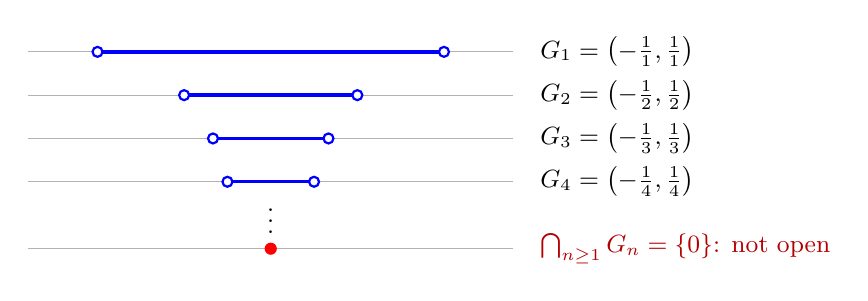
\begin{tikzpicture}[x=2.2cm, every node/.style={font=\small}]
	\foreach \n/\y in {1/0, 2/-0.55, 3/-1.1, 4/-1.65} {
		\draw[gray!60] (-1.4,\y) -- (1.4,\y);
		\draw[very thick, blue] ({-1/\n},\y) -- ({1/\n},\y);
		\draw[blue, thick, fill=white] ({-1/\n},\y) circle (1.8pt);
		\draw[blue, thick, fill=white] ({1/\n},\y) circle (1.8pt);
		\node[anchor=west] at (1.5,\y) {$G_{\n}=\left(-\tfrac1{\n},\tfrac1{\n}\right)$};
	}
	\node at (0,-2.05) {$\vdots$};
	\draw[gray!60] (-1.4,-2.5) -- (1.4,-2.5);
	\fill[red] (0,-2.5) circle (2.2pt);
	\node[anchor=west, red!70!black] at (1.5,-2.5) {$\bigcap_{n\ge1}G_n=\{0\}$: not open};
\end{tikzpicture}
\end{document}
